\section{Miner\'ia de texto}

Definimos miner\'ia de texto como  un proceso mediante el cual se buscan patrones destacados y nuevos conocimientos en un conjunto de textos, es decir, es el proceso encargado de descubrir conocimientos que no existen tal cual en ning\'un texto del conjunto seleccionado pero que destacan al relacionar el contenido de varios de ellos \cite{min1}. Es decir, b\'usqueda de regularidades o patrones que se encuentran en un texto, a partir de t\'ecnicas de aprendizaje autom\'atico. \\

Existen dos etapas principales dentro de este proceso: preprocesamiento y descubrimiento. Ver \ref{fig:mineriatexto}\\


\begin{figure}
\begin{center}
	\label{mineriatexto}
	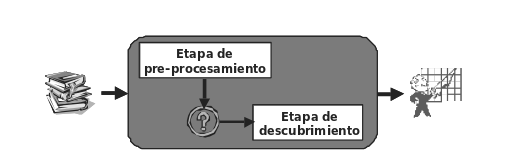
\includegraphics[scale=.6]{images/mintex}
	\label{fig:mineriatexto}
	\caption{Proceso de la Miner\'ia de texto}
\end{center}
\end{figure}


Todas las etapas est\'an muy interrelacionadas: la primera etapa condiciona el descubrimiento de los patrones que la miner\'ia de texto puede realizar. \\

El preprocesamiento consiste en transformar el texto en alg\'un tipo de estructura que nos facilite su an\'alisis.El proprocesamiento de textos implica la eliminaci\'on de informaci\'on textual que no ser\'a relevante para resolver la finalidad de nuestro proyecto \cite{min2}. Incluye la eliminaci\'on de palabras que no aportan informaci\'on, es decir, stop words, as\'i como la unificaci\'on de los t\'erminos restantes mediante t\'ecnicas de stemming.  Por otro lado en el descubrimiento se analiza la estructura ateriormente mencionada teniendo como objetivo descubrir patrones interesantes o conocimientos nuevos. \\

La miner\'ia de textos se utiliza principalmente para: extraer informaci\'on relevante de un documento, agregar y compartir informaci\'on autom\'aticamente, clasificar y organizar documentos seg\'un su contenido, organizar dep\'ositos para b\'usqueda y recuperaci\'on, clasificar textos e indexarlos en la web \cite{min3}.  \\

En el caso del presente trabajo terminal, se utiliz\'o la miner\'ia de datos con el af\'an de identificar patrones dentro de conversaciones que nos indiquen cuando estas pueden llegar a tener contenido sexual. 

\pagebreak




